\documentclass[UTF8,12pt]{ctexart}
\usepackage[a4paper,margin=24mm]{geometry}
\usepackage{amsmath,amssymb,bm,graphicx,adjustbox}
\newcommand{\fitmath}[1]{\begin{adjustbox}{max width=\linewidth}$\displaystyle #1$\end{adjustbox}}
\setlength{\parindent}{0pt}
\setlength{\parskip}{.7em}
\sloppy
\allowdisplaybreaks
\begin{document}
\section*{2009 年考研数学三 · 真题}
\subsection*{原 PDF 第 51 页}

\subsection*{2009年全国硕士研究生招生考试试题}

\subsection*{一、选择题（本题共8小题，每小题4分，共32分。在每小题给出的四个选项中，只有一项符合题目要求，把所选项前的字母填在题后的括号内。）}

（1）函数 \(\displaystyle f(x)=\dfrac{\displaystyle x-x^3}{\displaystyle \sin\pi x}\) 的可去间断点的个数为（　　）
（A）1。 （B）2。 （C）3。 （D）无穷多个。


（2）当 \(\displaystyle x\to0\) 时，\(\displaystyle f(x)=x-\sin ax\) 与 \(\displaystyle g(x)=x^2\ln(1-bx)\) 是等价无穷小量，则（　　）
（A）\(\displaystyle a=1,\allowbreak b=-\dfrac{\displaystyle 1}{\displaystyle 6}\)。 （B）\(\displaystyle a=1,\allowbreak b=\dfrac{\displaystyle 1}{\displaystyle 6}\)。 （C）\(\displaystyle a=-1,\allowbreak b=-\dfrac{\displaystyle 1}{\displaystyle 6}\)。 （D）\(\displaystyle a=-1,\allowbreak b=\dfrac{\displaystyle 1}{\displaystyle 6}\)。


（3）使不等式 \(\displaystyle \int_1^x\dfrac{\displaystyle \sin t}{\displaystyle t}\,dt>\ln x\) 成立的 \(\displaystyle x\) 的范围是（　　）
（A）\(\displaystyle (0,\allowbreak 1)\)。 （B）\(\displaystyle (1,\allowbreak \dfrac{\displaystyle \pi}{\displaystyle 2})\)。 （C）\(\displaystyle (\dfrac{\displaystyle \pi}{\displaystyle 2},\allowbreak \pi)\)。 （D）\(\displaystyle (\pi,\allowbreak +\infty)\)。


（4）设函数 \(\displaystyle y=f(x)\) 在区间 \(\displaystyle [-1,\allowbreak 3]\) 上的图形如图所示，则函数 \(\displaystyle F(x)=\displaystyle \int_0^x f(t)\,dt\) 的图形为（　　）。选项（A）、（B）、（C）、（D）见图。


\begin{center}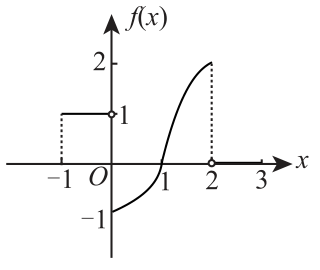
\includegraphics[width=.85\linewidth]{../assets/figures/page-051-06.png}\end{center}

\begin{center}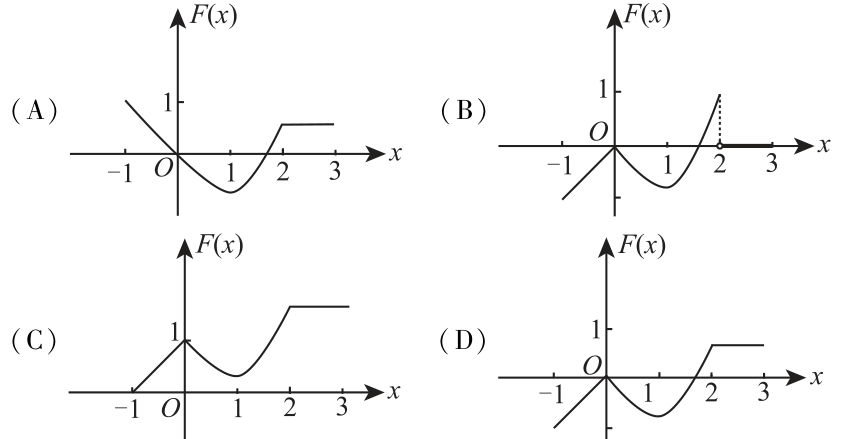
\includegraphics[width=.85\linewidth]{../assets/figures/page-051-07.png}\end{center}

（5）设 \(\displaystyle A,\allowbreak B\) 均为2阶方阵，\(\displaystyle A^*,\allowbreak B^*\) 分别为 \(\displaystyle A,\allowbreak B\) 的伴随矩阵。若 \(\displaystyle |A|=2,\allowbreak |B|=3\)，则分块矩阵 \(\displaystyle \begin{pmatrix}O&A\\B&O\end{pmatrix}\) 的伴随矩阵为（　　）
（A）\(\displaystyle \begin{pmatrix}O&3B^*\\2A^*&O\end{pmatrix}\)。 （B）\(\displaystyle \begin{pmatrix}O&2B^*\\3A^*&O\end{pmatrix}\)。
（C）\(\displaystyle \begin{pmatrix}O&3A^*\\2B^*&O\end{pmatrix}\)。 （D）\(\displaystyle \begin{pmatrix}O&2A^*\\3B^*&O\end{pmatrix}\)。


（6）设 \(\displaystyle A,\allowbreak P\) 均为3阶矩阵，\(\displaystyle P^{\mathrm T}\) 为 \(\displaystyle P\) 的转置矩阵，且 \(\displaystyle P^{\mathrm T}AP=\begin{pmatrix}1&0&0\\0&1&0\\0&0&2\end{pmatrix}\)。若 \(\displaystyle P=(\boldsymbol\alpha_1,\allowbreak \boldsymbol\alpha_2,\allowbreak \boldsymbol\alpha_3)\)，\(\displaystyle Q=\)


\clearpage

\subsection*{原 PDF 第 52 页}

\(\displaystyle (\boldsymbol\alpha_1+\boldsymbol\alpha_2,\allowbreak \boldsymbol\alpha_2,\allowbreak \boldsymbol\alpha_3)\)，则 \(\displaystyle Q^{\mathrm T}AQ\) 为（　　）
（A）\(\displaystyle \begin{pmatrix}2&1&0\\1&1&0\\0&0&2\end{pmatrix}\)。 （B）\(\displaystyle \begin{pmatrix}1&1&0\\1&2&0\\0&0&2\end{pmatrix}\)。
（C）\(\displaystyle \begin{pmatrix}2&0&0\\0&1&0\\0&0&2\end{pmatrix}\)。 （D）\(\displaystyle \begin{pmatrix}1&0&0\\0&2&0\\0&0&2\end{pmatrix}\)。


（7）设事件 \(\displaystyle A\) 与事件 \(\displaystyle B\) 互不相容，则（　　）
（A）\(\displaystyle P(\bar A\bar B)=0\)。 （B）\(\displaystyle P(AB)=P(A)P(B)\)。 （C）\(\displaystyle P(A)=1-P(B)\)。 （D）\(\displaystyle P(\bar A\cup\bar B)=1\)。


（8）设随机变量 \(\displaystyle X\) 与 \(\displaystyle Y\) 相互独立，且 \(\displaystyle X\) 服从标准正态分布 \(\displaystyle N(0,\allowbreak 1)\)，\(\displaystyle Y\) 的概率分布为 \(\displaystyle P\{Y=0\}=P\{Y=1\}=\dfrac{\displaystyle 1}{\displaystyle 2}\)。记 \(\displaystyle F_Z(z)\) 为随机变量 \(\displaystyle Z=XY\) 的分布函数，则函数 \(\displaystyle F_Z(z)\) 的间断点个数为（　　）
（A）0。 （B）1。 （C）2。 （D）3。


\subsection*{二、填空题（本题共6小题，每小题4分，共24分，把答案填在题中横线上。）}

（9）\(\displaystyle \lim_{x\to0}\dfrac{\displaystyle e-e^{\cos x}}{\displaystyle \sqrt[3]{1+x^2}-1}=\)\_\_\_\_\_\_。


（10）设 \(\displaystyle z=(x+e^y)^x\)，则 \(\displaystyle \left.\dfrac{\displaystyle \partial z}{\displaystyle \partial x}\right|_{(1,\allowbreak 0)}=\)\_\_\_\_\_\_。


（11）幂级数 \(\displaystyle \sum_{n=1}^{\infty}\dfrac{\displaystyle e^n-(-1)^n}{\displaystyle n^2}x^n\) 的收敛半径为\_\_\_\_\_\_。


（12）设某产品的需求函数为 \(\displaystyle Q=Q(p)\)，其对价格 \(\displaystyle p\) 的弹性 \(\displaystyle \varepsilon_p=0.2\)，则当需求量为10000件时，价格增加1元会使产品收益增加\_\_\_\_\_\_元。


（13）设 \(\displaystyle \boldsymbol\alpha=(1,\allowbreak 1,\allowbreak 1)^{\mathrm T},\allowbreak \boldsymbol\beta=(1,\allowbreak 0,\allowbreak k)^{\mathrm T}\)，若矩阵 \(\displaystyle \boldsymbol\alpha\boldsymbol\beta^{\mathrm T}\) 相似于 \(\displaystyle \begin{pmatrix}3&0&0\\0&0&0\\0&0&0\end{pmatrix}\)，则 \(\displaystyle k=\)\_\_\_\_\_\_。


（14）设 \(\displaystyle X_1,\allowbreak X_2,\allowbreak \ldots,\allowbreak X_m\) 为来自二项分布总体 \(\displaystyle B(n,\allowbreak p)\) 的简单随机样本，\(\displaystyle \bar X\) 和 \(\displaystyle S^2\) 分别为样本均值和样本方差。记统计量 \(\displaystyle T=\bar X-S^2\)，则 \(\displaystyle E(T)=\)\_\_\_\_\_\_。


\subsection*{三、解答题（本题共9小题，共94分，解答应写出文字说明、证明过程或演算步骤。）}

（15）（本题满分9分）求二元函数 \(\displaystyle f(x,\allowbreak y)=x^2(2+y^2)+y\ln y\) 的极值。


（16）（本题满分10分）计算不定积分 \(\displaystyle \int\ln\left(1+\sqrt{\dfrac{\displaystyle 1+x}{\displaystyle x}}\right)\,dx\;(x>0)\)。


\clearpage

\subsection*{原 PDF 第 53 页}

（17）（本题满分10分）计算二重积分 \(\displaystyle \iint_D(x-y)\,dx\,dy\)，其中 \(\displaystyle D=\{(x,\allowbreak y)\mid(x-1)^2+(y-1)^2\le2,\allowbreak \ y\ge x\}\)。


（18）（本题满分11分）
（I）证明拉格朗日中值定理：若函数 \(\displaystyle f(x)\) 在 \(\displaystyle [a,\allowbreak b]\) 上连续，在 \(\displaystyle (a,\allowbreak b)\) 内可导，则存在 \(\displaystyle \xi\in(a,\allowbreak b)\)，使得 \(\displaystyle f(b)-f(a)=f^{\prime}(\xi)(b-a)\)。
（II）证明：若函数 \(\displaystyle f(x)\) 在 \(\displaystyle x=0\) 处连续，在 \(\displaystyle (0,\allowbreak \delta)\;(\delta>0)\) 内可导，且 \(\displaystyle \lim_{x\to0^+}f^{\prime}(x)=A\)，则 \(\displaystyle f^{\prime}_+(0)\) 存在，且 \(\displaystyle f^{\prime}_+(0)=A\)。


（19）（本题满分10分）设曲线 \(\displaystyle y=f(x)\)，其中 \(\displaystyle f(x)\) 是可导函数，且 \(\displaystyle f(x)>0\)。已知曲线 \(\displaystyle y=f(x)\) 与直线 \(\displaystyle y=0,\allowbreak x=1\) 及 \(\displaystyle x=t\;(t>1)\) 所围成的曲边梯形绕 \(\displaystyle x\) 轴旋转一周所得的立体体积值是该曲边梯形面积值的 \(\displaystyle \pi t\) 倍，求该曲线的方程。


（20）（本题满分11分）设


\[\fitmath{\displaystyle A=\begin{pmatrix}1&-1&-1\\-1&1&1\\0&-4&-2\end{pmatrix},\quad\boldsymbol\xi_1=\begin{pmatrix}-1\\1\\-2\end{pmatrix}.}\]


（I）求满足 \(\displaystyle A\boldsymbol\xi_2=\boldsymbol\xi_1,\allowbreak \ A^2\boldsymbol\xi_3=\boldsymbol\xi_1\) 的所有向量 \(\displaystyle \boldsymbol\xi_2,\allowbreak \boldsymbol\xi_3\)；
（II）对（I）中的任意向量 \(\displaystyle \boldsymbol\xi_2,\allowbreak \boldsymbol\xi_3\)，证明 \(\displaystyle \boldsymbol\xi_1,\allowbreak \boldsymbol\xi_2,\allowbreak \boldsymbol\xi_3\) 线性无关。


\clearpage

\subsection*{原 PDF 第 54 页}

（21）（本题满分11分）设二次型 \(\displaystyle f(x_1,\allowbreak x_2,\allowbreak x_3)=ax_1^2+ax_2^2+(a-1)x_3^2+2x_1x_3-2x_2x_3\)。
（I）求二次型 \(\displaystyle f\) 的矩阵的所有特征值；
（II）若二次型 \(\displaystyle f\) 的规范形为 \(\displaystyle y_1^2+y_2^2\)，求 \(\displaystyle a\) 的值。


（22）（本题满分11分）设二维随机变量 \(\displaystyle (X,\allowbreak Y)\) 的概率密度为


\[\fitmath{\displaystyle f(x,y)=\begin{cases}e^{-x},&0<y<x,\\0,&\text{其他}.\end{cases}}\]


（I）求条件概率密度 \(\displaystyle f_{Y\mid X}(y\mid x)\)；
（II）求条件概率 \(\displaystyle P\{X\le1\mid Y\le1\}\)。


（23）（本题满分11分）袋中有1个红球、2个黑球与3个白球。现有放回地从袋中取两次，每次取一个球。以 \(\displaystyle X,\allowbreak Y,\allowbreak Z\) 分别表示两次取球所取得的红球、黑球与白球的个数。
（I）求 \(\displaystyle P\{X=1\mid Z=0\}\)；
（II）求二维随机变量 \(\displaystyle (X,\allowbreak Y)\) 的概率分布。


\clearpage
\end{document}
